% Supplementary material for the JSTARS manuscript. Build: tectonic -X compile supplement.tex
\documentclass[journal,onecolumn]{IEEEtran}
\usepackage{iftex}
\ifPDFTeX\usepackage[utf8]{inputenc}\fi
\usepackage[T1]{fontenc}
\usepackage{amsmath,amssymb,textcomp,graphicx,booktabs,array}
\usepackage{float}
\usepackage[hidelinks]{hyperref}
\usepackage{newunicodechar}
\newunicodechar{−}{\ensuremath{-}}
\newunicodechar{Δ}{\ensuremath{\Delta}}
\newunicodechar{ρ}{\ensuremath{\rho}}
\newunicodechar{→}{\ensuremath{\rightarrow}}
\newunicodechar{±}{\ensuremath{\pm}}
\newunicodechar{≥}{\ensuremath{\geq}}
\newunicodechar{≤}{\ensuremath{\leq}}
\newunicodechar{–}{--}
\newunicodechar{—}{---}
\graphicspath{{../../figures/}}
\newcommand{\iouf}{IoU$_\text{flood}$}
\newcommand{\ci}[2]{[#1,\,#2]}
\renewcommand{\thetable}{S\arabic{table}}
\renewcommand{\thefigure}{S\arabic{figure}}

\begin{document}
\title{Supplementary Material for ``Terrain Helps SAR Flood Mapping on New Floods''}
\author{Jeremy~Ky, Bao~Duong, and~Rich~Nguyen}
\maketitle
\sloppy

All CIs are 95\%. Unless stated otherwise, multi-seed CIs are two-way bootstraps over seeds or training
draws and test events. ``Unseen activations'' are GEOID-Flood test events whose activation does not
appear in GEOID-Flood train. Every number is produced by the scripts listed in the repository's
\texttt{REPRODUCE.md}.

\section*{Leave-one-event-out on Sen1Floods11}

\begin{table}[H]
\caption{Leave-one-event-out on Sen1Floods11 (11 events, 3 seeds; 5 where noted). Mean held-out event
IoU and paired difference to the SAR-only model, with 95\% CI over events; $p$: Wilcoxon signed-rank over
events. The 5-seed SAR-only mean is 0.566; the ResNet-34 SAR-only mean is 0.584.}
\centering
\resizebox{\ifdim\width>\linewidth\linewidth\else\width\fi}{!}{%
\begin{tabular}{@{}lcccc@{}}
\toprule
Variant & IoU & Δ vs SAR only & $p$ & Improved \\
\midrule
SAR only (VV, VH) & 0.571 & & & \\
+ HAND input & 0.589 & +0.018 [−0.000, +0.035] & 0.12 & 8/11 \\
+ HAND input, 5 seeds & 0.591 & +0.025 [+0.005, +0.045] & 0.083 & 8/11 \\
+ HAND, DEM, slope inputs & 0.584 & +0.012 [−0.012, +0.033] & 0.21 & 8/11 \\
+ monotonicity loss & 0.569 & −0.002 [−0.010, +0.005] & 0.64 & 4/11 \\
+ ceiling loss & 0.571 & −0.001 [−0.010, +0.007] & 0.97 & 6/11 \\
+ HAND input + monotonicity & 0.588 & +0.017 [+0.000, +0.033] & 0.12 & 7/11 \\
+ monotonicity, 30-m stride, $w{=}1$ & 0.570 & −0.002 [−0.007, +0.004] & 0.47 & 4/11 \\
+ monotonicity, 30-m stride, $w{=}10$ & 0.571 & −0.001 [−0.006, +0.004] & 0.77 & 5/11 \\
+ HAND + mono.\ 30 m, $w{=}1$ (vs + HAND) & 0.596 & +0.006 [−0.002, +0.016] & 0.28 & 6/11 \\
+ HAND + mono.\ 30 m, $w{=}10$ (vs + HAND) & 0.595 & +0.006 [−0.004, +0.015] & 0.054 & 9/11 \\
ResNet-34: + HAND input & 0.600 & +0.017 [−0.001, +0.033] & 0.12 & 8/11 \\
\bottomrule
\end{tabular}}
\end{table}

With 11 events, which events gain is not reproducible across backbones (Spearman $\rho = 0.07$ between
the U-Net and ResNet-34 per-event gains).

\section*{Terrain and permanent-water ablation with GEOID-Flood training}

\begin{table}[H]
\caption{Terrain and permanent-water ablation with GEOID-Flood training (unseen activations; 20 events: 5
draws, 159 events: 3 seeds). Paired Δ with two-way 95\% CIs.}
\centering
\resizebox{\ifdim\width>\linewidth\linewidth\else\width\fi}{!}{%
\begin{tabular}{@{}lcccc@{}}
\toprule
Comparison & Training events & Flood, event-mean Δ & Flood, pooled Δ & All water, event-mean Δ \\
\midrule
DEM + slope vs SAR & 20 & +0.021 [+0.002, +0.044] & +0.046 [+0.016, +0.078] & +0.064 [+0.024, +0.110] \\
HAND vs SAR & 20 & +0.032 [+0.004, +0.065] & +0.062 [+0.019, +0.111] & +0.072 [+0.026, +0.124] \\
HAND + DEM + slope vs SAR & 20 & +0.027 [+0.000, +0.058] & +0.060 [+0.019, +0.099] & +0.076 [+0.030, +0.129] \\
HAND vs DEM + slope & 20 & +0.011 [−0.005, +0.032] & +0.015 [−0.021, +0.049] & +0.009 [−0.011, +0.029] \\
DEM + slope vs SAR & 159 & −0.010 [−0.027, +0.007] & −0.003 [−0.035, +0.026] & +0.017 [−0.005, +0.038] \\
HAND vs SAR & 159 & −0.001 [−0.019, +0.016] & +0.011 [−0.017, +0.037] & +0.023 [+0.004, +0.045] \\
HAND + DEM + slope vs SAR & 159 & +0.003 [−0.015, +0.020] & +0.014 [−0.014, +0.037] & +0.031 [+0.011, +0.054] \\
HAND vs DEM + slope & 159 & +0.009 [−0.013, +0.034] & +0.014 [−0.017, +0.051] & +0.007 [−0.008, +0.027] \\
\midrule
JRC vs SAR & 20 & −0.007 [−0.045, +0.024] & +0.001 [−0.059, +0.040] & +0.072 [+0.005, +0.154] \\
HAND vs JRC & 20 & +0.039 [+0.010, +0.072] & +0.061 [+0.015, +0.113] & +0.000 [−0.044, +0.041] \\
HAND + JRC vs HAND & 20 & −0.013 [−0.033, +0.003] & −0.013 [−0.043, +0.014] & +0.024 [−0.005, +0.062] \\
JRC vs SAR & 159 & −0.054 [−0.089, −0.024] & −0.078 [−0.132, −0.033] & −0.003 [−0.034, +0.028] \\
HAND vs JRC & 159 & +0.052 [+0.020, +0.089] & +0.088 [+0.043, +0.140] & +0.027 [−0.005, +0.060] \\
HAND + JRC vs HAND & 159 & −0.012 [−0.031, +0.001] & −0.013 [−0.029, +0.000] & +0.006 [−0.012, +0.025] \\
\bottomrule
\end{tabular}}
\end{table}

HAND's edge over DEM and slope with GEOID-Flood training is not significant under the two-way bootstrap;
with test events alone resampled, the 20-event flood CI, \ci{+0.001}{+0.022}, just excludes zero. Adding
DEM and slope to HAND adds nothing (flood −0.005 \ci{−0.015}{+0.005} at 20 events). In the Sen1Floods11
transfer, adding the JRC layer to HAND changes little (CIs over test events: +0.007 \ci{+0.002}{+0.014} all water; −0.002
\ci{−0.005}{+0.002} flood).

\section*{TerraMind with GEOID-Flood training}

\begin{table}[H]
\caption{TerraMind (TM) and U-Net, ± HAND, with GEOID-Flood training (unseen activations, event-mean IoU,
two-way 95\% CIs; number of improved events where given).}
\centering
\resizebox{\ifdim\width>\linewidth\linewidth\else\width\fi}{!}{%
\begin{tabular}{@{}llcc@{}}
\toprule
Comparison & Labels & 20 events (5 draws) & 159 events (3 seeds) \\
\midrule
TM + HAND − TM & flood & +0.031 [+0.001, +0.072], 34/38 & +0.002 [−0.015, +0.027] \\
TM + HAND − TM & all water & +0.049 [+0.006, +0.106], 36/39 & +0.005 [−0.017, +0.032] \\
U-Net + HAND − U-Net & flood & +0.032 [+0.004, +0.065] & −0.001 [−0.019, +0.016] \\
TM − U-Net (SAR only) & flood & +0.016 [−0.007, +0.042] & +0.005 [−0.010, +0.019] \\
TM − U-Net (SAR only) & all water & +0.052 [+0.008, +0.109] & +0.019 [+0.002, +0.038] \\
U-Net + HAND − TM & flood & +0.016 [−0.007, +0.045] & −0.006 [−0.029, +0.020] \\
U-Net + HAND − TM & all water & +0.020 [−0.012, +0.059] & +0.005 [−0.022, +0.032] \\
\bottomrule
\end{tabular}}
\end{table}

At 159 events TerraMind loses the all-water HAND gain the U-Net keeps (+0.005 vs.\ +0.023). Under the
GEOID-Flood protocol (pooled \iouf{}, unseen activations): at 20 events TerraMind goes from 0.443 to 0.480
with HAND (+0.040 \ci{+0.011}{+0.070}; held-out 2026 events +0.037 \ci{+0.003}{+0.080}); TerraMind alone
vs.\ U-Net alone +0.060 \ci{+0.005}{+0.112}, and the U-Net with HAND (0.448) equals TerraMind alone. At 159
events: 0.517 → 0.519, +0.001 \ci{−0.024}{+0.029} (held-out +0.013 \ci{−0.008}{+0.029}); TerraMind alone
beats the U-Net, +0.042 \ci{+0.011}{+0.071}.

\section*{Learning curve, equal-tiles control and the confirmation test}

\begin{table}[H]
\caption{HAND gain against the number of training events with every subset cut to 500 tiles (flooded water
only, 38 unseen test activations, 3 exploratory draws). Two-way 95\% CIs.}
\centering
\resizebox{\ifdim\width>\linewidth\linewidth\else\width\fi}{!}{%
\begin{tabular}{@{}lcccc@{}}
\toprule
Training events & Event-mean IoU, SAR → + HAND & Δ (95\% CI) & Pooled IoU, SAR → + HAND & Δ (95\% CI) \\
\midrule
10 & 0.380 → 0.366 & −0.014 [−0.043, +0.007] & 0.530 → 0.527 & −0.003 [−0.057, +0.040] \\
20 & 0.364 → 0.376 & +0.012 [+0.001, +0.025] & 0.511 → 0.549 & +0.038 [+0.009, +0.072] \\
40 & 0.359 → 0.370 & +0.011 [−0.013, +0.037] & 0.495 → 0.531 & +0.037 [−0.011, +0.094] \\
80 & 0.367 → 0.377 & +0.010 [−0.007, +0.026] & 0.514 → 0.546 & +0.031 [−0.001, +0.068] \\
159 & 0.381 → 0.381 & +0.000 [−0.012, +0.012] & 0.536 → 0.555 & +0.019 [−0.009, +0.052] \\
\bottomrule
\end{tabular}}
\end{table}

\begin{figure}[H]
\centering
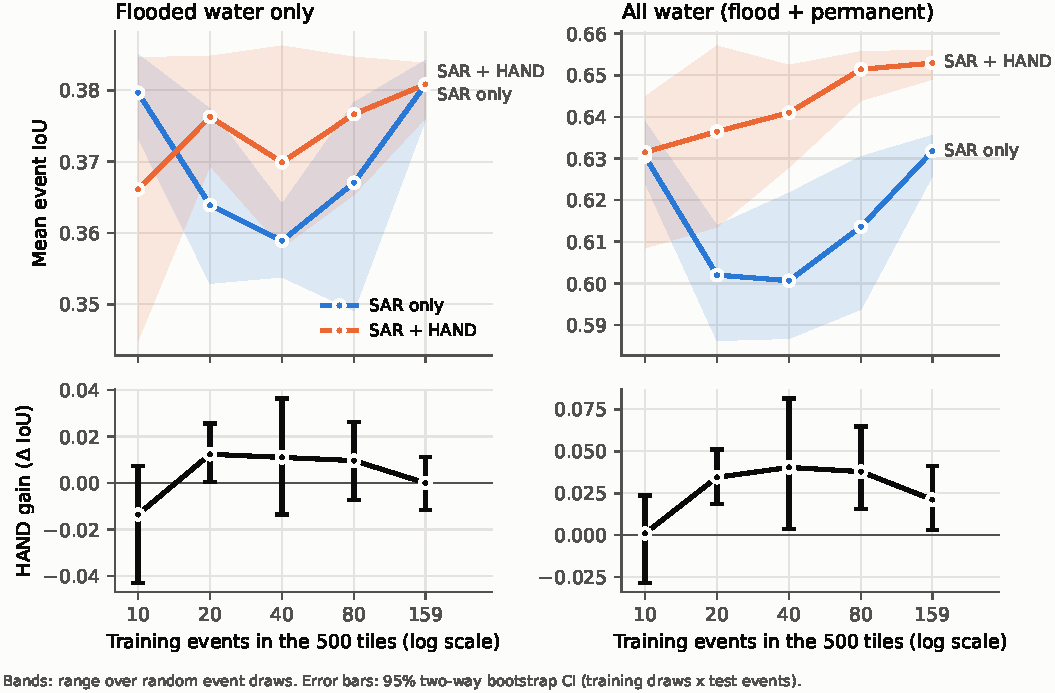
\includegraphics[width=0.75\textwidth]{fig_tile_control.pdf}
\caption{As the main learning-curve figure, with every training subset cut to 500 tiles spread evenly over
its events (3 exploratory draws).}
\end{figure}

\begin{table}[H]
\caption{Event-mean IoU regressed on $\log_2$ events and $\log_2$ tiles over all 38 exploratory training
draws (unseen activations; two-way 95\% CIs).}
\centering
\resizebox{\ifdim\width>\linewidth\linewidth\else\width\fi}{!}{%
\begin{tabular}{@{}llcc@{}}
\toprule
Outcome & Labels & Per doubling of events & Per doubling of tiles \\
\midrule
SAR-only IoU & flood & +0.007 [+0.001, +0.015] & −0.001 [−0.006, +0.004] \\
SAR-only IoU & all water & +0.014 [+0.004, +0.028] & −0.004 [−0.014, +0.003] \\
SAR + HAND IoU & flood & +0.004 [−0.001, +0.009] & +0.000 [−0.003, +0.004] \\
SAR + HAND IoU & all water & +0.009 [+0.003, +0.016] & −0.002 [−0.007, +0.001] \\
HAND gain & flood & −0.003 [−0.010, +0.003] & +0.001 [−0.003, +0.007] \\
HAND gain & all water & −0.005 [−0.016, +0.003] & +0.002 [−0.005, +0.009] \\
\bottomrule
\end{tabular}}
\end{table}

\emph{Learning curve, all water} (unseen activations, 39 events; event-mean Δ, then pooled Δ): 10 events
+0.050 \ci{+0.021}{+0.092}, +0.074 \ci{+0.028}{+0.148}; 20: +0.072 \ci{+0.026}{+0.124}, +0.101
\ci{+0.029}{+0.189}; 40: +0.044 \ci{+0.015}{+0.076}, +0.064 \ci{+0.019}{+0.132}; 80: +0.026
\ci{+0.008}{+0.047}, +0.048 \ci{+0.007}{+0.106}; 159: +0.023 \ci{+0.004}{+0.045}, +0.050
\ci{+0.003}{+0.118}. A linear fit of the gain on log events is not significant, because the gain rises
from 10 to 20 events and then falls. Threshold-free, event-mean flood AP gains on the exploratory draws are
+0.028 \ci{+0.016}{+0.041} at 20 events, +0.023 \ci{+0.009}{+0.039} at 40 and −0.000 \ci{−0.014}{+0.012} at
159 (CIs over test events only).

\emph{Confirmation test.} The contrast CIs resample test events, with the contrast averaged over draws.
All water: gains +0.035, +0.019 and +0.020 at 20, 40 and 159 events, contrast +0.007 \ci{−0.005}{+0.019},
$p = 0.37$. Secondary analysis on all test events, including those sharing activations with training:
flood +0.006 \ci{−0.000}{+0.013}, $p = 0.043$; all water +0.010 \ci{+0.001}{+0.019}, $p = 0.091$. Post hoc
AP version on the confirmation draws: flood gains +0.017, +0.000 and +0.004, contrast +0.004
\ci{−0.006}{+0.018}, $p = 0.49$; all water $p = 0.75$. Per-draw gains of the 40- and 159-event
confirmation draws were seen before the analysis ran, but the test was fixed and committed beforehand.

\emph{159 events, more detail.} All-water event-mean AP on unseen activations rises by (CI over test events) +0.011
\ci{+0.001}{+0.022}; flood AP pooled 0.730 → 0.732. Change detection with the pre-event image: on the
held-out 2026 events HAND gives +0.021 \ci{−0.004}{+0.053} at 159 events (single image −0.017), and +0.006
(change detection) vs.\ +0.016 (single image) at 20 events, all CIs including zero.

\section*{Relief gate}

\begin{table}[H]
\caption{Relief gate: gated minus ungated HAND model, \iouf{} under the GEOID-Flood protocol, unseen
activations, two-way 95\% CIs.}
\centering
\resizebox{\ifdim\width>\linewidth\linewidth\else\width\fi}{!}{%
\begin{tabular}{@{}lcc@{}}
\toprule
Training events & Pooled & Event-mean \\
\midrule
20 (5 draws) & −0.016 [−0.047, +0.001] & −0.002 [−0.005, +0.000] \\
159 (3 seeds) & −0.003 [−0.007, +0.001] & −0.002 [−0.006, +0.000] \\
\bottomrule
\end{tabular}}
\end{table}

131 of 2,635 test tiles are flat (36 on unseen activations). On the held-out 2026 events the gate changes
\iouf{} by −0.001 (20 events) and +0.003 (159), CIs including zero. The change-detection and TerraMind
pairs behave the same (all CIs include zero; $|\Delta| \le 0.008$ except change detection at 20 events,
pooled −0.013 \ci{−0.055}{+0.012}). Exploratory thresholds, unseen pooled at 20 events: 1\,m −0.015, 2\,m
−0.016, 5\,m −0.022 \ci{−0.053}{−0.002}. The gate recovers part of the EMSR419 loss when the post-event map
alone is scored (159 events, shared activations, flood labels: pooled Δ vs.\ SAR only −0.030 → −0.012), but
that event motivated the rule, and under the protocol the gate lowers pooled IoU on the same events (−0.009
\ci{−0.023}{−0.000}).

\section*{HAND dropout}

\begin{table}[H]
\caption{HAND dropout ($p = 0.5$) minus no dropout, unseen activations, two-way 95\% CIs. Tail: events
where the HAND model is worse than SAR only by more than 0.02 IoU (draw-averaged), without → with
dropout. Sen1Floods11-trained models are scored on all 77/79 GEOID-Flood test events.}
\centering
\resizebox{\ifdim\width>\linewidth\linewidth\else\width\fi}{!}{%
\begin{tabular}{@{}lcccc@{}}
\toprule
Training & Event-mean Δ, flood & Event-mean Δ, all water & Protocol pooled \iouf{} Δ & Tail (flood / protocol) \\
\midrule
Sen1Floods11, 11 events (3 seeds) & −0.008 [−0.016, −0.001] & −0.020 [−0.036, −0.009] & −0.027 [−0.060, −0.002] & 7 → 6 / 4 → 6 \\
GEOID, 20 events (5 draws) & +0.001 [−0.017, +0.019] & −0.017 [−0.042, +0.005] & −0.009 [−0.049, +0.024] & 2 → 4 / 1 → 2 \\
GEOID, 159 events (3 seeds) & +0.001 [−0.015, +0.017] & −0.013 [−0.033, +0.006] & −0.013 [−0.036, +0.012] & 8 → 4 / 5 → 2 \\
\bottomrule
\end{tabular}}
\end{table}

With 11 training events dropout removes 0.008 of HAND's 0.032 flood event-mean gain, 0.020 of 0.061 for all
water and 0.027 of 0.072 under the protocol. With few events the tail does not shrink (11 events) or grows
(20). At 159 events the summed loss over tail events falls from −0.32 to −0.06, and the event-mean protocol
gain over SAR only from +0.013 to +0.004. The Swedish tile (EMSR280\_1-0, Sen1Floods11-trained): SAR only
0.61, HAND 0.30, HAND with dropout 0.46 (3 seeds); the Swedish event, all water: 0.663 → 0.592
(Sen1Floods11), 0.622 → 0.527 (20 events), 0.688 → 0.552 (159 events).

\section*{Where the gain occurs}

\begin{table}[H]
\caption{HAND gain by pixel stratum for the Sen1Floods11-trained U-Net on GEOID-Flood test (3 seeds; flood: 77
events, all water: 79). Pooled IoU SAR → SAR + HAND, pooled Δ with two-way 95\% CIs over seeds and the events
with water in the stratum, and false-alarm rate FP/(FP + TN) in percent (identical in both label modes).
The IoU and false-alarm columns pool all events; Δ averages per-seed differences over the events with water
in the stratum, so it need not equal the difference of the IoU columns. Moss and lichen and snow and ice
(under 5 events, negligible area) are omitted.}
\centering
\resizebox{\ifdim\width>\linewidth\linewidth\else\width\fi}{!}{%
\begin{tabular}{@{}lccccc@{}}
\toprule
 & \multicolumn{3}{c}{Flooded water only} & \multicolumn{2}{c}{All water} \\
Stratum & IoU & Δ pooled & False alarm (\%) & IoU & Δ pooled \\
\midrule
HAND 0-1 m & 0.475 → 0.514 & +0.040 [+0.004, +0.095] & 5.68 → 5.45 & 0.758 → 0.791 & +0.033 [+0.012, +0.063] \\
HAND 1-2 m & 0.295 → 0.386 & +0.091 [+0.021, +0.154] & 2.68 → 1.35 & 0.360 → 0.446 & +0.087 [+0.025, +0.149] \\
HAND 2-5 m & 0.263 → 0.353 & +0.089 [+0.030, +0.154] & 1.58 → 0.65 & 0.311 → 0.380 & +0.069 [+0.019, +0.130] \\
HAND 5-10 m & 0.200 → 0.276 & +0.061 [+0.012, +0.100] & 0.77 → 0.19 & 0.231 → 0.272 & +0.041 [+0.007, +0.085] \\
HAND 10-20 m & 0.089 → 0.127 & +0.026 [−0.033, +0.113] & 0.54 → 0.05 & 0.147 → 0.188 & +0.024 [−0.016, +0.078] \\
HAND $>$20 m & 0.018 → 0.034 & +0.015 [−0.021, +0.083] & 0.62 → 0.02 & 0.033 → 0.049 & +0.014 [−0.022, +0.060] \\
\midrule
Slope 0-2\textdegree & 0.454 → 0.517 & +0.063 [+0.018, +0.116] & 4.59 → 3.78 & 0.748 → 0.796 & +0.048 [+0.019, +0.082] \\
Slope 2-5\textdegree & 0.335 → 0.389 & +0.054 [+0.024, +0.087] & 1.29 → 0.85 & 0.427 → 0.485 & +0.058 [+0.034, +0.084] \\
Slope 5-10\textdegree & 0.231 → 0.283 & +0.051 [+0.023, +0.071] & 0.76 → 0.43 & 0.346 → 0.402 & +0.056 [+0.030, +0.079] \\
Slope 10-20\textdegree & 0.144 → 0.197 & +0.052 [+0.028, +0.078] & 0.43 → 0.17 & 0.247 → 0.294 & +0.047 [+0.023, +0.074] \\
Slope $>$20\textdegree & 0.021 → 0.072 & +0.054 [+0.028, +0.081] & 1.38 → 0.14 & 0.065 → 0.174 & +0.109 [+0.069, +0.147] \\
\midrule
tree cover & 0.241 → 0.311 & +0.069 [+0.026, +0.112] & 0.67 → 0.29 & 0.258 → 0.311 & +0.053 [+0.024, +0.083] \\
shrubland & 0.624 → 0.639 & +0.015 [−0.021, +0.073] & 0.27 → 0.18 & 0.680 → 0.694 & +0.014 [−0.017, +0.063] \\
grassland & 0.538 → 0.581 & +0.043 [+0.023, +0.063] & 2.26 → 1.59 & 0.545 → 0.587 & +0.042 [+0.023, +0.063] \\
cropland & 0.491 → 0.589 & +0.099 [+0.019, +0.193] & 2.45 → 1.98 & 0.500 → 0.597 & +0.097 [+0.019, +0.196] \\
built-up & 0.089 → 0.117 & +0.028 [+0.005, +0.058] & 0.54 → 0.44 & 0.127 → 0.149 & +0.023 [+0.001, +0.048] \\
bare & 0.088 → 0.118 & +0.031 [+0.019, +0.076] & 31.08 → 22.95 & 0.138 → 0.183 & +0.046 [+0.027, +0.099] \\
herbaceous wetland & 0.450 → 0.452 & +0.002 [−0.019, +0.022] & 11.86 → 11.64 & 0.584 → 0.589 & +0.006 [−0.012, +0.021] \\
permanent water & 0.227 → 0.225 & −0.002 [−0.009, +0.005] & 32.35 → 34.21 & 0.933 → 0.957 & +0.024 [+0.009, +0.051] \\
mangroves (5/7 events) & 0.205 → 0.177 & −0.030 [−0.042, +0.033] & 0.37 → 0.31 & 0.588 → 0.528 & −0.060 [−0.088, −0.038] \\
\bottomrule
\end{tabular}}
\end{table}

\emph{Country clusters} (pre-registered \#8, seeds 0--2). Event-mean HAND gain of the Sen1Floods11-trained
U-Net with the CI resampling events and seeds, then countries (34--35, with all their events) and seeds: flood
+0.032 \ci{+0.018}{+0.050} and \ci{+0.017}{+0.051}; all water +0.061 \ci{+0.040}{+0.087} and
\ci{+0.039}{+0.089}. ResNet-34: flood +0.022 \ci{+0.006}{+0.039} and \ci{+0.005}{+0.039}; all water +0.036
\ci{+0.012}{+0.065} and \ci{+0.014}{+0.064}.

\section*{HAND perturbations (mechanism tests)}

\begin{table}[H]
\caption{Pre-registered HAND perturbations, Sen1Floods11-trained U-Net (3 seeds), all 77/79 GEOID-Flood test
events: event-mean and pooled Δ with two-way 95\% CIs. Shifts are applied in both image axes; the blur is
Gaussian with the given $\sigma$.}
\centering
\resizebox{\ifdim\width>\linewidth\linewidth\else\width\fi}{!}{%
\begin{tabular}{@{}lcccc@{}}
\toprule
 & \multicolumn{2}{c}{Flooded water only} & \multicolumn{2}{c}{All water} \\
Comparison & Event-mean Δ & Pooled Δ & Event-mean Δ & Pooled Δ \\
\midrule
Correct HAND − SAR only & +0.032 [+0.018, +0.050] & +0.074 [+0.037, +0.120] & +0.061 [+0.040, +0.086] & +0.059 [+0.032, +0.089] \\
Shifted 100 m − SAR only & +0.025 [+0.012, +0.041] & +0.070 [+0.036, +0.113] & +0.031 [+0.012, +0.052] & +0.047 [+0.024, +0.072] \\
Shifted 500 m − SAR only & +0.003 [−0.011, +0.018] & +0.050 [+0.020, +0.083] & −0.003 [−0.019, +0.013] & +0.014 [−0.013, +0.041] \\
Blurred 250 m − SAR only & −0.001 [−0.015, +0.014] & +0.030 [+0.003, +0.053] & −0.034 [−0.058, −0.010] & −0.019 [−0.066, +0.021] \\
Other event's HAND (test) − SAR only & −0.061 [−0.081, −0.041] & −0.033 [−0.086, +0.013] & −0.122 [−0.151, −0.095] & −0.095 [−0.151, −0.040] \\
Trained with other events' HAND − SAR only & −0.005 [−0.015, +0.006] & −0.014 [−0.037, +0.024] & −0.001 [−0.021, +0.015] & −0.007 [−0.032, +0.021] \\
\midrule
Shifted 100 m − correct HAND & −0.007 [−0.014, −0.001] & −0.003 [−0.013, +0.007] & −0.030 [−0.042, −0.019] & −0.012 [−0.023, −0.004] \\
Shifted 500 m − correct HAND & −0.029 [−0.044, −0.016] & −0.024 [−0.044, −0.008] & −0.063 [−0.085, −0.046] & −0.045 [−0.078, −0.023] \\
Blurred 250 m − correct HAND & −0.033 [−0.050, −0.020] & −0.044 [−0.100, −0.004] & −0.094 [−0.121, −0.070] & −0.078 [−0.141, −0.033] \\
Other event's HAND (test) − correct HAND & −0.093 [−0.119, −0.067] & −0.106 [−0.175, −0.048] & −0.182 [−0.220, −0.148] & −0.154 [−0.225, −0.094] \\
Trained with other events' HAND − correct HAND & −0.037 [−0.053, −0.022] & −0.088 [−0.122, −0.047] & −0.062 [−0.084, −0.042] & −0.066 [−0.104, −0.034] \\
\bottomrule
\end{tabular}}
\end{table}

\section*{Same tiles with their event in training or held out}

\begin{table}[H]
\caption{The 90 tiles of Sen1Floods11's official test split (10 events), scored by the official-split models,
trained on other tiles of the same events, and by the leave-one-event-out models that held the tile's event
out (pre-registered \#9; all water, hand labels; 5 seeds in each setting). Per event: IoU pooled over the
event's test tiles, mean over seeds; gain: SAR + HAND minus SAR only from the same seed. Summary rows:
two-way 95\% CIs (events shared by both settings, seeds resampled within each).}
\centering
\resizebox{\ifdim\width>\linewidth\linewidth\else\width\fi}{!}{%
\begin{tabular}{@{}lrcccccc@{}}
\toprule
 & & \multicolumn{3}{c}{Event in training (official split)} & \multicolumn{3}{c}{Event held out (LOEO)} \\
Event & Tiles & SAR & + HAND & Gain & SAR & + HAND & Gain \\
\midrule
Ghana & 11 & 0.554 & 0.544 & −0.010 & 0.529 & 0.537 & +0.007 \\
India & 14 & 0.696 & 0.707 & +0.011 & 0.681 & 0.697 & +0.016 \\
Mekong & 6 & 0.854 & 0.850 & −0.004 & 0.855 & 0.855 & +0.001 \\
Nigeria & 4 & 0.885 & 0.881 & −0.005 & 0.887 & 0.887 & +0.000 \\
Pakistan & 6 & 0.217 & 0.235 & +0.017 & 0.229 & 0.262 & +0.034 \\
Paraguay & 14 & 0.649 & 0.663 & +0.014 & 0.578 & 0.682 & +0.103 \\
Somalia & 6 & 0.465 & 0.427 & −0.039 & 0.491 & 0.498 & +0.007 \\
Spain & 6 & 0.716 & 0.725 & +0.010 & 0.727 & 0.718 & −0.008 \\
Sri Lanka & 9 & 0.843 & 0.873 & +0.030 & 0.845 & 0.878 & +0.033 \\
USA & 14 & 0.549 & 0.538 & −0.011 & 0.492 & 0.472 & −0.019 \\
\midrule
Event mean & & & & +0.001 [−0.021, +0.019] & & & +0.017 [−0.004, +0.043] \\
Pooled over the 90 tiles & & & & +0.008 [−0.007, +0.018] & & & +0.024 [−0.007, +0.053] \\
\bottomrule
\end{tabular}}
\end{table}

Held out minus in training: event-mean +0.016 \ci{−0.009}{+0.045} (primary), pooled +0.016
\ci{−0.013}{+0.046}; the held-out gain is larger on 8 of the 10 events. The hypothesis (a CI above zero) is
not supported. Paraguay contributes most: with its event held out, the SAR-only model loses 0.07 IoU on its
tiles and the HAND model none.

\section*{Physics losses and HAND post-masks on the Sen1Floods11 transfer}

\begin{table}[H]
\caption{Physics losses and HAND post-masks, trained on the 11 Sen1Floods11 events, all 77/79 GEOID-Flood test
events (pre-registered \#10; losses: 3 seeds, masks: 5 seeds; two-way 95\% CIs). A mask at $t$ sets predicted
water above $t$ metres HAND to dry (in both images under the protocol); no retraining.}
\label{tab:transferlossmask}
\centering
\resizebox{\ifdim\width>\linewidth\linewidth\else\width\fi}{!}{%
\begin{tabular}{@{}lccc@{}}
\toprule
Comparison & Flood, event-mean Δ & All water, event-mean Δ & Protocol pooled Δ \\
\midrule
SAR only + monotonicity loss − SAR only & +0.000 [−0.007, +0.008] & −0.011 [−0.021, −0.003] & −0.003 [−0.018, +0.008] \\
SAR only + ceiling loss − SAR only & +0.008 [−0.004, +0.024] & +0.006 [−0.011, +0.025] & +0.003 [−0.017, +0.032] \\
SAR only + monotonicity, 30-m stride, $w{=}1$ − SAR only & +0.002 [−0.004, +0.007] & +0.001 [−0.009, +0.009] & +0.002 [−0.019, +0.020] \\
SAR only + monotonicity, 30-m stride, $w{=}10$ − SAR only & +0.009 [+0.003, +0.017] & +0.002 [−0.014, +0.014] & +0.008 [−0.001, +0.017] \\
\midrule
SAR only + mask 5\,m − SAR only & +0.015 [+0.007, +0.025] & +0.021 [+0.008, +0.037] & +0.010 [+0.002, +0.020] \\
SAR only + mask 10\,m − SAR only & +0.013 [+0.006, +0.021] & +0.020 [+0.009, +0.035] & +0.010 [+0.005, +0.017] \\
SAR only + mask 15\,m − SAR only & +0.011 [+0.005, +0.019] & +0.019 [+0.008, +0.033] & +0.008 [+0.004, +0.014] \\
SAR only + mask 20\,m − SAR only & +0.010 [+0.005, +0.017] & +0.018 [+0.008, +0.031] & +0.007 [+0.003, +0.011] \\
SAR + HAND + mask 5\,m − SAR + HAND & +0.003 [−0.001, +0.012] & +0.003 [−0.002, +0.012] & −0.003 [−0.007, −0.000] \\
SAR + HAND + mask 10\,m − SAR + HAND & +0.004 [+0.000, +0.012] & +0.004 [−0.000, +0.013] & +0.000 [−0.001, +0.001] \\
SAR + HAND + mask 15\,m − SAR + HAND & +0.003 [+0.000, +0.011] & +0.005 [+0.000, +0.014] & +0.000 [−0.000, +0.001] \\
SAR + HAND + mask 20\,m − SAR + HAND & +0.003 [+0.000, +0.011] & +0.005 [+0.000, +0.013] & +0.000 [+0.000, +0.001] \\
\midrule
SAR + HAND − SAR only (Table III) & +0.032 [+0.019, +0.048] & +0.063 [+0.044, +0.085] & +0.074 [+0.035, +0.126] \\
SAR + HAND − (SAR only + mask 5\,m)$^a$ & +0.017 [+0.005, +0.032] & +0.042 [+0.025, +0.062] & +0.064 [+0.025, +0.115] \\
SAR + HAND − (SAR only + mask 20\,m)$^a$ & +0.023 [+0.010, +0.038] & +0.045 [+0.029, +0.063] & +0.067 [+0.028, +0.119] \\
\bottomrule
\end{tabular}}
\\[2pt]\raggedright\footnotesize $^a$Exploratory (not pre-registered).
\end{table}

Unlike in leave-one-event-out, where the 15-m mask changed held-out IoU by less than 0.003, every mask
improves the SAR-only model on the external events, on 52--71 of the 77/79 events, by removing water
predicted on high ground, which the HAND input also removes. The input gains two to three and a half times as much in
event-mean IoU and seven to ten times as much under the protocol, and masking the HAND model adds almost
nothing. Of the losses, only monotonicity at a 30-m stride and weight 10 improves the SAR-only model with a
CI above zero, in flooded-water IoU (on 53 of 77 events), by about as much as a 20-m mask; the stride-1
monotonicity loss lowers all-water IoU (on 55 of 79 events).

\section*{Do the reference labels encode a HAND mask?}

The Global Flood Monitoring product excludes pixels with HAND of 10\,m or more (15\,m in earlier versions,
after Twele et al.)~\cite{gfm2025pdd,twele2016sentinel1}. If the reference labels had been made with such an
exclusion, a model given HAND could gain by reproducing it. GEOID-Flood test labels are CEMS rapid-mapping
delineations, whose documentation describes semi-automatic classification and photo-interpretation and no
terrain mask~\cite{joubertboitat2020cemsrm}; Sen1Floods11's hand labels were drawn from Sentinel-1 and
Sentinel-2 imagery alone~\cite{bonafilia2020sen1floods11}. Table~\ref{tab:labelhand} checks the labels
directly (pre-registered \#13, descriptive). A cut-off is flagged when an event has at least 1,000
labelled-water pixels within 1\,m below a threshold, at least 1,000 valid pixels within 1\,m above it, and no
labelled water there; no event in either dataset is flagged at any threshold. Of the 72 flood events with at
least 1\% of their area above 15\,m HAND, 56 have labelled flood water there. The 99th percentile of
labelled-water HAND has a median over events of 6.5\,m (flooded water; range 0.2--87.5\,m), 6.0\,m (all
water; 0.2--40.2\,m) and 5.0\,m (Sen1Floods11; 1.2--10.2\,m). GEOID-Flood labels thus put more water at high
HAND than Sen1Floods11's hand labels do, not less.

\begin{table}[H]
\caption{Labelled water above HAND thresholds, per event. Events: events with at least 1\% of their valid
area above the threshold; none above: of these, events with no labelled water above it; median share: median
over all events of the share of labelled water above the threshold; cut-offs: see text.}
\label{tab:labelhand}
\centering
\resizebox{\ifdim\width>\linewidth\linewidth\else\width\fi}{!}{%
\begin{tabular}{@{}lccccccccc@{}}
\toprule
 & \multicolumn{3}{c}{GEOID-Flood, flooded (77 events)} & \multicolumn{3}{c}{GEOID-Flood, all water (79)} &
 \multicolumn{3}{c}{Sen1Floods11, hand labels (11)} \\
HAND & Events / none above & Median share & Cut-offs & Events / none above & Median share & Cut-offs &
Events / none above & Median share & Cut-offs \\
\midrule
5\,m & 77 / 3 & 1.51\% & 0 & 79 / 1 & 1.24\% & 0 & 11 / 0 & 0.93\% & 0 \\
10\,m & 73 / 12 & 0.28\% & 0 & 75 / 5 & 0.23\% & 0 & 10 / 0 & 0.05\% & 0 \\
15\,m & 72 / 16 & 0.15\% & 0 & 74 / 11 & 0.09\% & 0 & 10 / 2 & 0.01\% & 0 \\
20\,m & 71 / 21 & 0.05\% & 0 & 72 / 16 & 0.06\% & 0 & 10 / 2 & 0.01\% & 0 \\
\bottomrule
\end{tabular}}
\end{table}

\section*{Change detection with the pre-event image}

GEOID-Flood provides a pre-event Sentinel-1 image for every tile, so a model can be given both images at
once. Operationally, Sentinel-1's routine acquisitions usually supply a recent pre-event image of the same
orbit, but seasonal changes in vegetation and soil moisture between the two dates add their own errors. We train the same U-Net on [VV, VH, VV\textsubscript{pre}, VH\textsubscript{pre}] (± HAND) to predict
flooded water directly, with permanent water and background as negatives, i.e., GEOID-Flood's flood class.
All 8,712 training tiles have a pre-event image; requiring both images removes 0.8\% of valid pixels. It
is scored on exactly the tiles and pixels of the protocol-matched single-image numbers, so the rows of
Table~\ref{tab:cd} are directly comparable.

\begin{table}[H]
\caption{HAND gain with and without the pre-event image (unseen activations; pooled \iouf{} under the
GEOID-Flood protocol, mean over draws/seeds; Δ from confusion counts averaged over draws/seeds, two-way
95\% CI; last column event-mean Δ).}
\label{tab:cd}
\centering
\resizebox{\ifdim\width>\linewidth\linewidth\else\width\fi}{!}{%
\begin{tabular}{@{}lccccc@{}}
\toprule
Model & Events & SAR & + HAND & Δ pooled (95\% CI) & Δ ev. \\
\midrule
Single image, differenced & 20 & 0.382 & 0.448 & +0.066 [+0.019, +0.111] & +0.036 \\
Change detection & 20 & 0.404 & 0.426 & +0.024 [−0.037, +0.085] & +0.000 \\
Single image, differenced & 159 & 0.475 & 0.496 & +0.021 [−0.001, +0.043] & +0.013 \\
Change detection & 159 & 0.463 & 0.491 & +0.029 [−0.011, +0.057] & +0.005 \\
\bottomrule
\end{tabular}}
\end{table}

A trained change model is no better than differencing two single-image maps (without HAND: −0.014 at 159
events, +0.020 at 20, CIs including zero), but it is much less sensitive to
which 20 events it is trained on (standard deviation over draws 0.041 vs.\ 0.090). With the pre-event
image, HAND matters less at 20 events (+0.024 vs.\ +0.066, no longer significant) and about as much at 159
(+0.029 vs.\ +0.021); the event-mean gains are near zero. Plausibly the pre-event image supplies part of what
HAND supplies with few training events: which dark, smooth surfaces were already there before the flood.

\section*{Pre-registration record}

\begin{table}[H]
\caption{Pre-registered analyses: when each plan was committed (git commit time, UTC$-$5) and where. Plans,
deviations and outcomes are in the repository's \texttt{PREREGISTRATIONS.md}. Analyses 9--15 respond to an
external review of a draft of this paper; what had been seen before they were fixed is listed there.}
\label{tab:prereg}
\centering
\resizebox{\ifdim\width>\linewidth\linewidth\else\width\fi}{!}{%
\begin{tabular}{@{}rllll@{}}
\toprule
\# & Analysis & Paper & Fixed & Commit \\
\midrule
1 & HAND gain vs.\ training events at 500 tiles (confirmation test) & V-F & 2026-11-12 07:48 & c5616fa$^a$ \\
2 & Relief gate & V-G & 2026-11-21 11:03 & 8b9a359$^a$ \\
3 & HAND dropout & V-G & 2026-11-21 11:37 & 6eb1e69, b08389c$^a$ \\
4 & Terrain ablation on the Sen1Floods11 transfer & V-C & 2026-11-21 21:29 & 58cc5ad$^a$ \\
5 & TerraMind on the Sen1Floods11 transfer & V-E & 2026-11-21 21:31 & 6f7aacf$^a$ \\
6--8 & HAND perturbations; errors by stratum; country-cluster bootstrap & V-B, V-D & 2026-11-22 21:52 & 106706e \\
9--15 & Same tiles in/out of training; losses and masks on the transfer; split overlap; TerraMind
learning rate; label check; fixed-epoch learning curve; five seeds & V, S & 2026-11-23 20:01 & 014c1af \\
\bottomrule
\end{tabular}}
\\[2pt]\raggedright\footnotesize $^a$Development repository, whose history is available from the authors on
request; other commits are in the public repository.
\end{table}

\section*{Additional figures}

\begin{figure}[H]
\centering
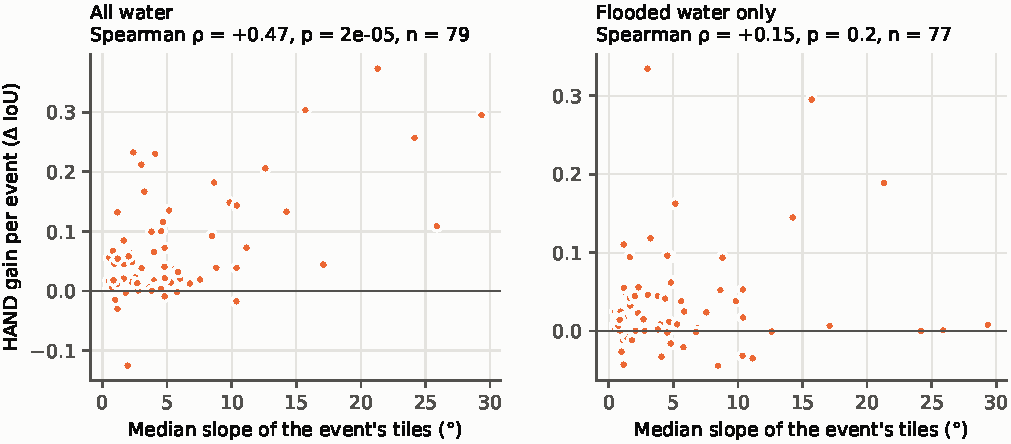
\includegraphics[width=0.7\textwidth]{fig_gain_vs_terrain.pdf}
\caption{Per-event HAND gain (mean over 5 seeds) of the Sen1Floods11-trained U-Net on GEOID-Flood test events against the
event's median slope, for all water (left, 79 events) and flooded water only (right, 77 events). The
all-water gain grows with terrain variation.}
\end{figure}

\begin{figure}[H]
\centering
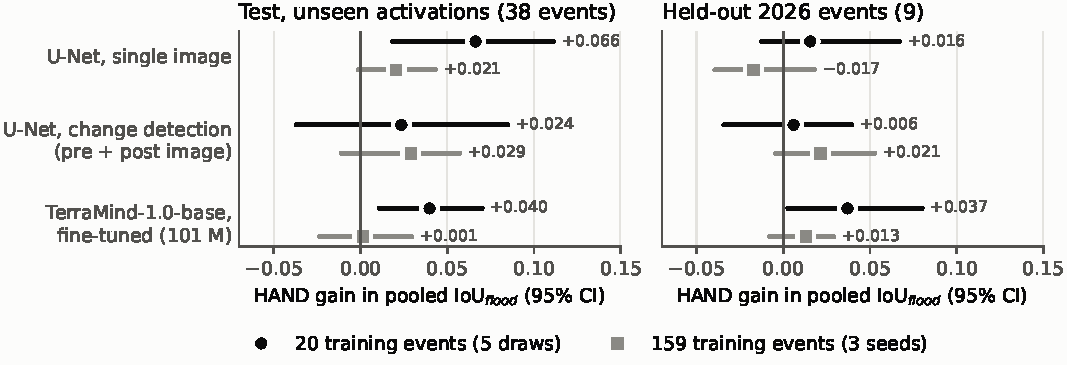
\includegraphics[width=0.7\textwidth]{fig_backbones.pdf}
\caption{HAND gain under the GEOID-Flood protocol (pooled \iouf{}, two-way 95\% CIs) for the single-image
U-Net, the change-detection U-Net and TerraMind, trained on 20 or 159 GEOID-Flood events; unseen test
activations (left) and held-out 2026 events (right).}
\end{figure}

\bibliographystyle{IEEEtran}
\bibliography{refs}

\end{document}
